


\subsection{Output Analysis of $S(d)$}


  \subsubsection{Periodic Boundary Conditions}

      \begin{figure}
         \centering
         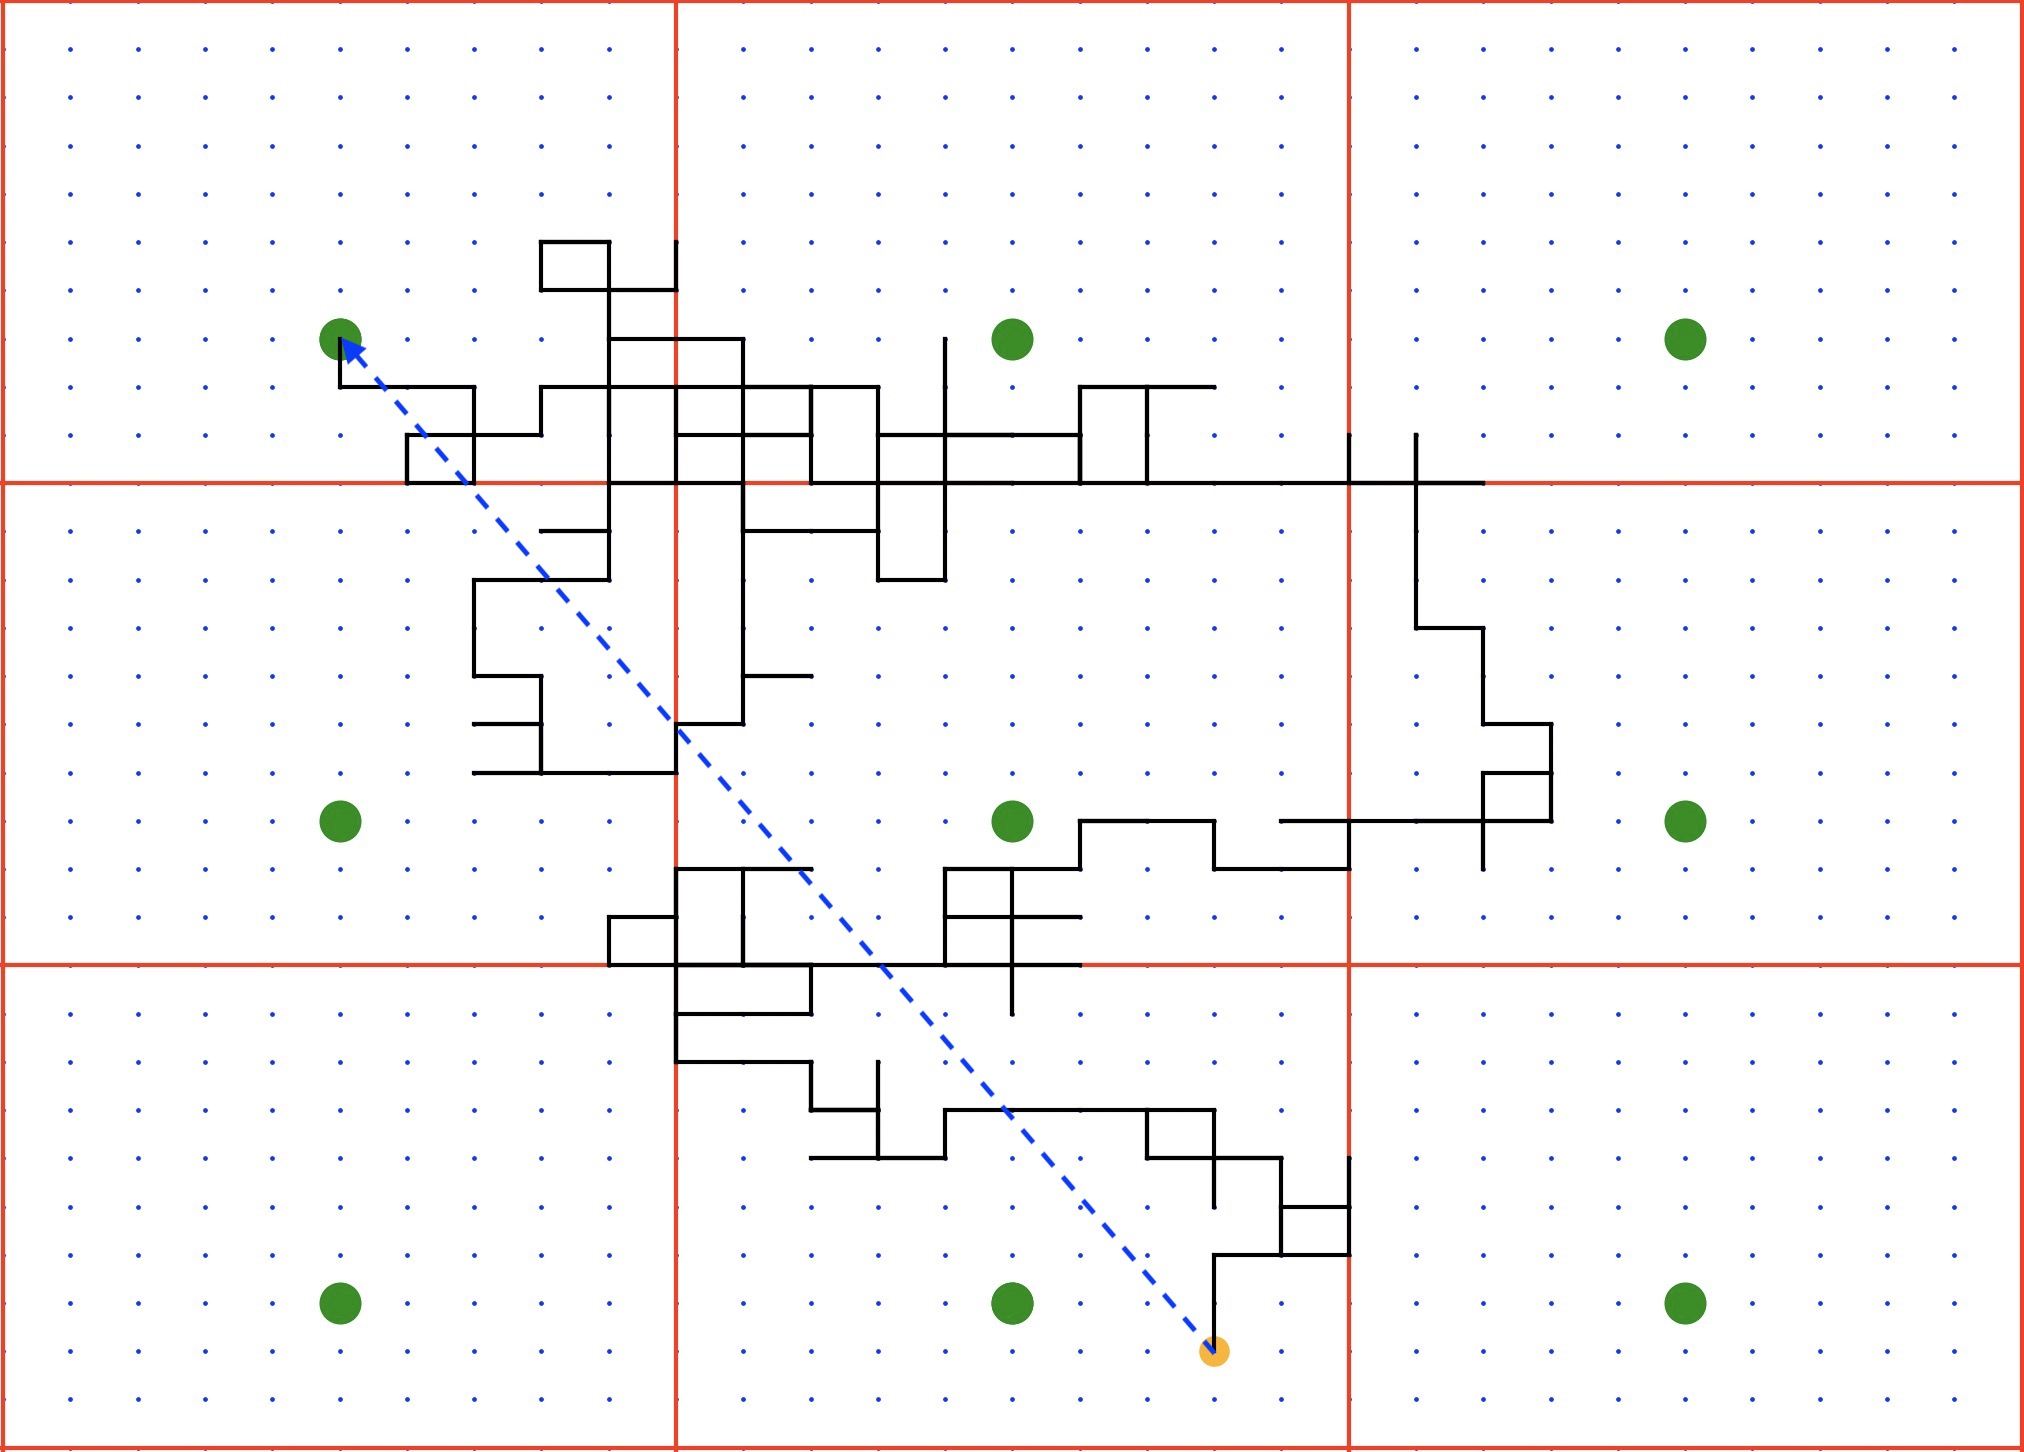
\includegraphics[width=\textwidth]{lrw_perodic_bc.png}
         \caption{This plane is constructed by choosing a primitive
           cell with four red sides and a green point and replicating
           it infinitely to tile the whole $2-$ dimensional
           space. Moreover, there has no overlaps and voids between
           copies of the cell. A particle initially started LRWs from
           the orange site and be absorbed by any of the green points.
           To ensure smoothness and consistency, if the particle
           leaves the cell through one edge, it will appear in the
           adjacent cell with the same velocity. The black line
           segments show the particle's random trajectories, and the
           length of the blue dotted arrow is defined as its
           displacement.}
         \label{fig:pbc_lrws}
      \end{figure}


      In this thesis, periodic boundary conditions (PBCs) are employed
      to minimize the influence of images'
      edges. Fig.~\ref{fig:pbc_lrws} is a simplest example of
      implementing PBCs in the Euclidean plane $E^2$ and tracks the
      trajectory of a particle undergoing LRWs. 




    \subsubsection{Relationship between $n$ and $d$}

     In this section, the displacement of a particle, $d$, is the
     shortest distance from the initial to the stop position in the
     infinite tiling plane. In theory, the mean square displacement
     (MSD) of $N$ Brownian particles at $n-$th step in $2-$dimensional
     space is defined as

     \begin{equation}\label{eq:mds_N}
       MSD = \langle \lvert \bm{r}(n) \lvert^2 \rangle = \frac{1}{N} \sum^{N}_{i=1} (\bm{s}_{i}(n) - \bm{s}_{i}(0))^2 = 4Dn
     \end{equation}
     where the subscript, $i$, refers to each particle for which the
     MSD is calculated. $\bm{s}_{i}(n)$ and $\bm{s}_{i}(0)$ are the
     $i-$th particle positions at $n-$th step and at the initial time,
     respectively. $D$ is diffusion coefficient which is related to
     the variance of the independent displacements of the
     particle. In the simulation, $D$ equals $1$.
     
      
      \begin{figure}
         \centering
         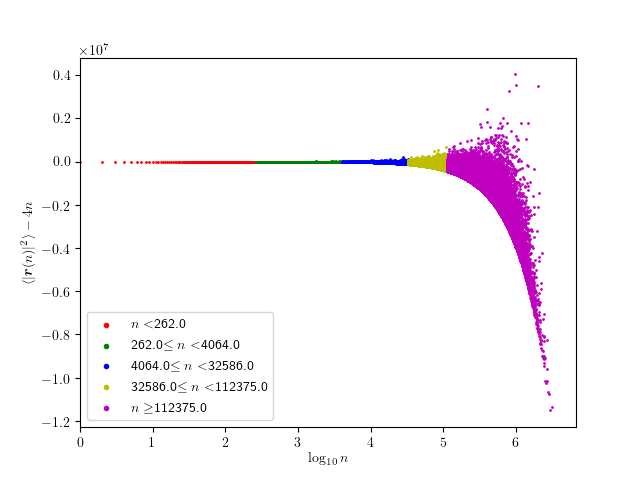
\includegraphics[width=\textwidth]{G_1_L_3_msd_n.png}
         \caption{Particles in $G_1L_3$ are divided into several
           subgroups based on various intervals of steps, and their
           colours are as identical as the segments in
           Fig.~\ref{fig:steps_seg_curve_G_1_L_3}.}
         \label{fig:G_1_L_3_msd_n}
      \end{figure}


     Eq.~\ref{eq:mds_N} indicates a linear relationship between the
     mean square displacement of the particle and the number of
     steps. It is a feature of the normal diffusive
     behavior. Fig.~\ref{fig:G_1_L_3_msd_n} shows how the difference
     between MSD of the particle and $4n$ varying over $\log_{10}n$ in
     LRWs. When $n \leq 4064.0$, the variation is not
     equal to $0$ with larger fluctuation, which implies that blue,
     yellow, and pink particles undergo anomalous diffusion
     process. In other words,

     \begin{equation}\label{eq:anomalous_diffusion}
       \langle \lvert \bm{r}(n) \lvert^2 \rangle \propto n^{\gamma}
     \end{equation}
     where $\gamma \ne 1$. In Fig.~\ref{fig:steps_seg_curve_G_1_L_3},
     negative variation implies $\gamma < 1$ called sub-diffusion
     process, while positive value denotes $\gamma > 1$ named
     super-diffusion.

     
      \begin{figure}
         \centering
         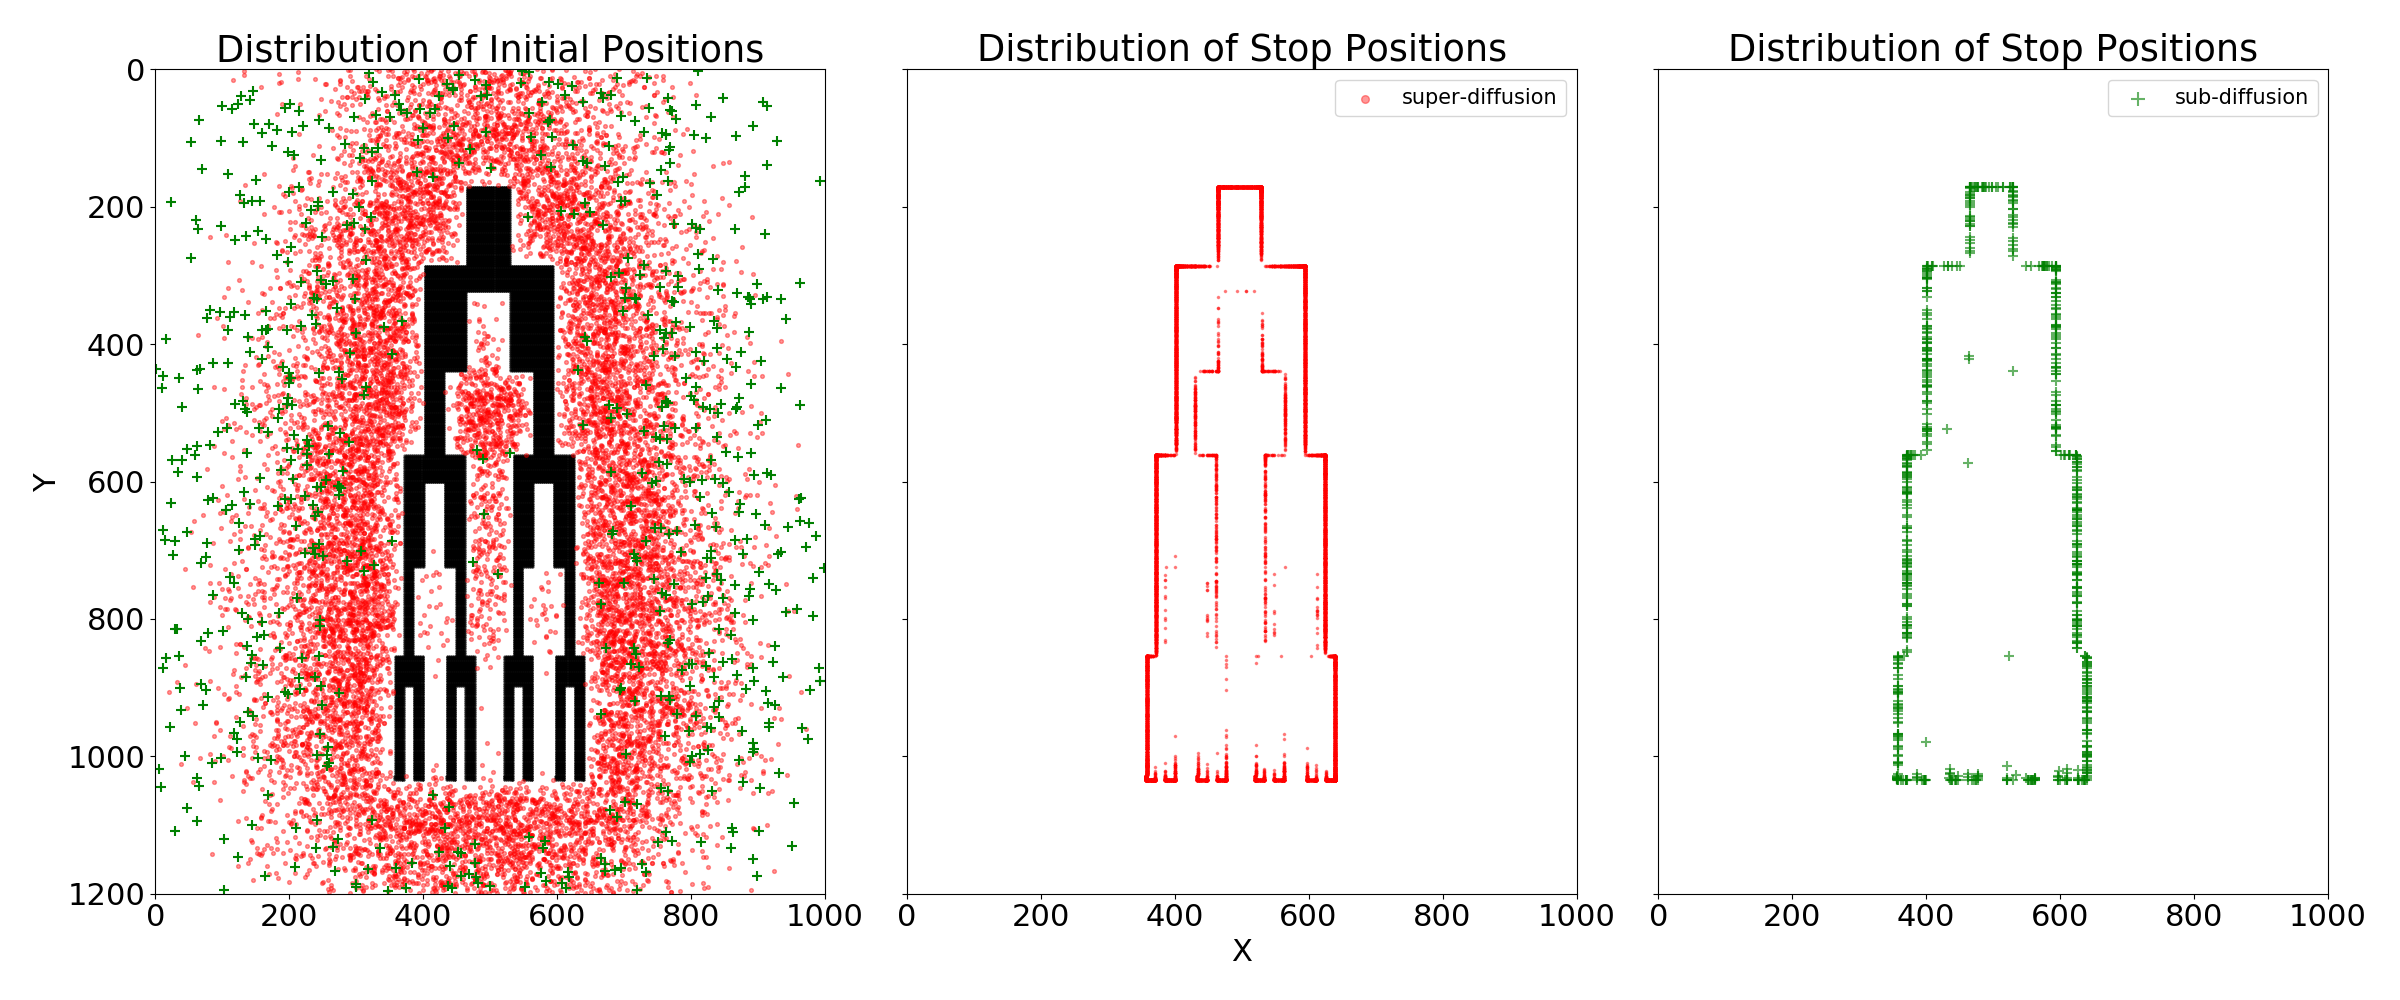
\includegraphics[width=\textwidth]{G_1_L_3_steps_blue_initial_stop_pos_var.png}
         \caption{In the left figure, $696$ dark blue pluses refer to
           super-diffusion particles, which are distributed closer and
           more concentrated to the fringe of the branching
           structure. $15198$ pale blue points represent sub-diffusion
           particles and scatter mainly around the edges of the
           image. In-between the branches, there has only six
           super-diffusion particles and an enormous amount of
           sub-diffusion ones. The middle and right depict the stop
           positions for super and sub-diffusion particles,
           respectively, coloured by a perceptually uniform sequential
           colormap based on their maximum displacement in the tiling
           space.}
         \label{fig:G_1_L_3_var_initial_stop_pos}
      \end{figure}

      To understand the underlying mechanism of the anomalous-type
      diffusion process, initial and stop positions of particles in
      Fig.~\ref{fig:G_1_L_3_steps_blue_initial_pos_distribution},
      whose steps ranged from $4064$ to $32586$, are illustrated in
      Fig.~\ref{fig:G_1_L_3_var_initial_stop_pos}. Suppose particles
      are trapped in the narrow space in-between the branches or
      initially start LRWs near the branching structure. In that case,
      their movements will be restricted because of the nearby
      absorbing boundary condition, causing the sub-diffusion
      phenomenon. As shown in the middle subplot of
      Fig.~\ref{fig:G_1_L_3_var_initial_stop_pos}, the maximum
      displacement of sub-diffusion particles is less than
      $200$. There also have exceptional circumstances that $6$
      particles, in-between the limbs, undergo super-diffusion since
      they can explore a large portion of space within a predefined
      range of steps, as shown in the right subfigure of
      Fig.~\ref{fig:G_1_L_3_var_initial_stop_pos}. Generally,
      particles around the edges of the image will be more likely to
      pass through the periodic boundary, reappear in the adjacent
      cell, and continue LRWs with the same velocity until hitting the
      absorbing boundary, which results in large displacement and the
      super-diffusion process.
      
      

      \subsubsection{Estimated Survival Functions}
      
      \begin{figure}
        \centering
        \begin{subfigure}[b]{0.45\textwidth}
          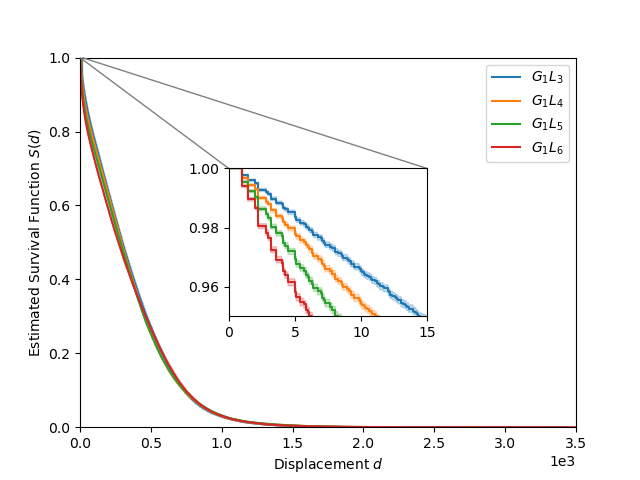
\includegraphics[width=\textwidth]{G_1_unwrap_disp_sf.png}
          \caption{}
          \label{fig:sf_g1_branch_disp}
        \end{subfigure}
        \hfill
        \begin{subfigure}[b]{0.45\textwidth}
          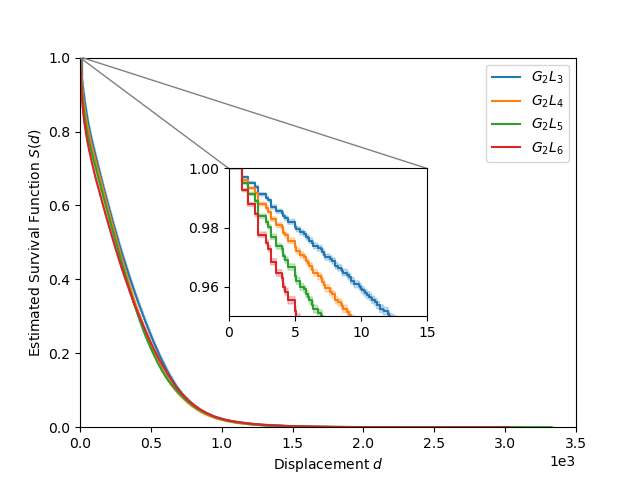
\includegraphics[width=\textwidth]{G_2_unwrap_disp_sf.png}
          \caption{}
          \label{fig:sf_g2_branch_disp}
        \end{subfigure}
        \caption{(a) and (b) are the estimated survival functions
          associated with particles' displacement in LRWs in $G_1$ and
          $G_2$, respectively.}
        \label{fig:sf_branch_disp}
      \end{figure}

      Similar to Fig.~\ref{fig:sf_branch_steps}, it is arduous to
      detect the variation among the survival curves by eyes. However,
      their short-term behaviours can be enlarged in insets in
      Fig.~\ref{fig:sf_branch_disp}, and we can conclude that the
      bigger $L_i$, $i=3, ..., 6$, leads to faster decay of survival
      function. The survival curve is analyzed segment by segment
      based on particles' initial and stop positions, shown in
      Fig.~\ref{fig:G_1_L_3_disp_red_initial_pos_distribution},
      Fig.~\ref{fig:G_1_L_3_disp_green_initial_pos_distribution},
      Fig.~\ref{fig:G_1_L_3_disp_blue_initial_pos_distribution},
      Fig.~\ref{fig:G_1_L_3_disp_yellow_initial_pos_distribution}, and
      Fig.~\ref{fig:G_1_L_3_disp_pink_initial_pos_distribution}, for
      the further understanding.
      


      \begin{figure}
         \centering
         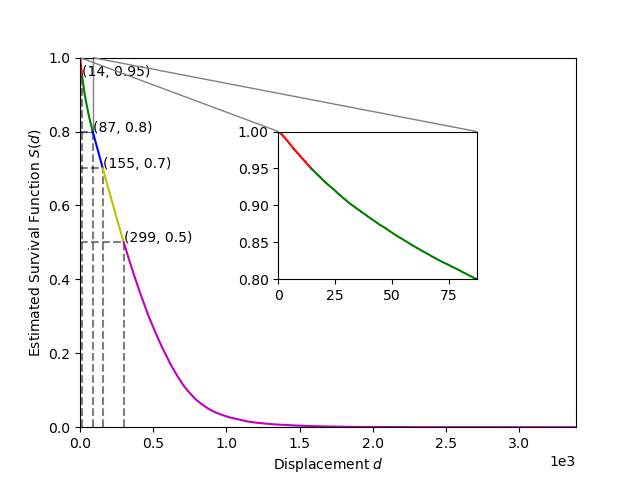
\includegraphics[width=\textwidth]{unwrap_disp_seg_curve_G_1_L_3.png}
         \caption{The estimated survival function is separated into
           five coloured segments based on various intervals of
           displacement. Less than $1\%$ of particles will survive
           when their displacement beyond the height of the image.}
         \label{fig:disp_seg_curve_G_1_L_3}
      \end{figure}

      
       \begin{figure}
         \centering
         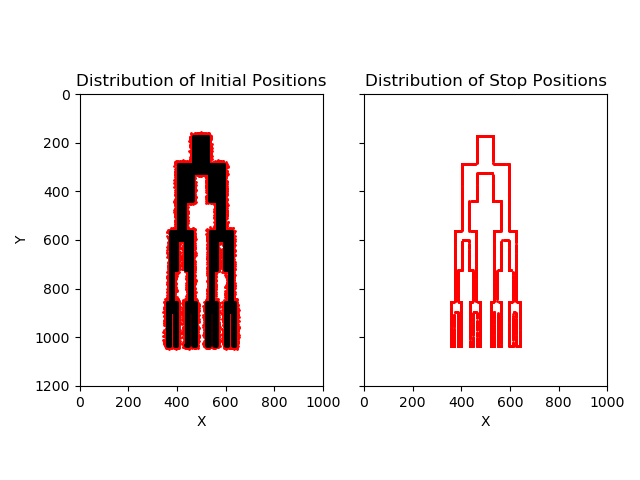
\includegraphics[width=\textwidth]{G_1_L_3_unwrap_disp_red_initial_pos_distribution.png}
         \caption{Five percent of particles are distributed in a tight
           and slender band, with a width of $14$, surrounding the
           branch structure. The area between the bottom and middle
           branches is filled with red particles, which implies the
           vertical spacing between those branches is less than or
           equal to $14$. The right subfigure shows that red particles
           can characterize the entire boundary of the target object.}
         \label{fig:G_1_L_3_disp_red_initial_pos_distribution}
       \end{figure}


       \begin{figure}
         \centering
         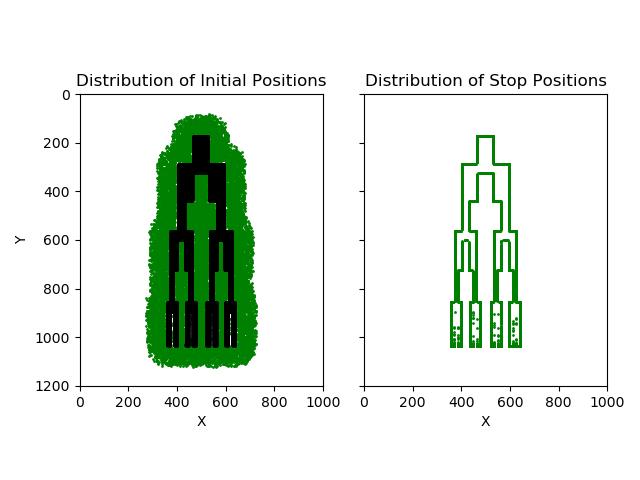
\includegraphics[width=\textwidth]{G_1_L_3_unwrap_disp_green_initial_pos_distribution.png}
         \caption{Compared with
           Fig.~\ref{fig:G_1_L_3_disp_red_initial_pos_distribution},
           fifteen percent of particles can fill the space between the
           branches and occupy the region surrounding the object in
           the shape of a wider band (i.e. with the width
           $73$). Moreover, green particles can not carry the detailed
           information of the boundary of bottom branches.}
         \label{fig:G_1_L_3_disp_green_initial_pos_distribution}
       \end{figure}


        \begin{figure}
         \centering
         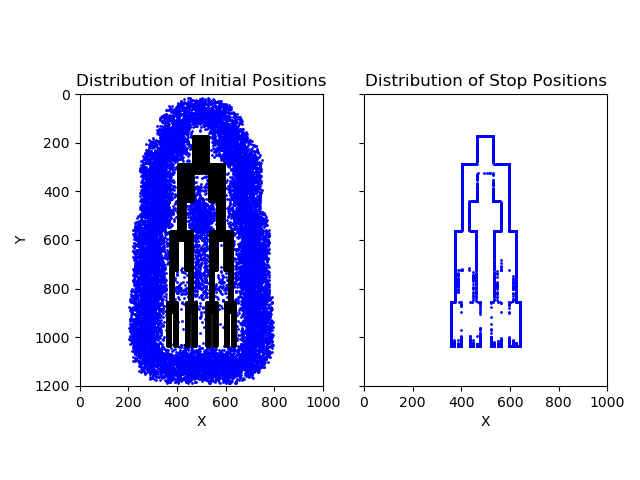
\includegraphics[width=\textwidth]{G_1_L_3_unwrap_disp_blue_initial_pos_distribution.png}
         \caption{Ten percent of particles, whose distances in LRWs
           range between $87$ and $155$, are distributed a little far
           away from the branching structure. Besides, some of them
           are located in the top space between the thick
           branches. Also, the top and bottom of the blue particles
           band are adjacent to the edge of the image. In comparison
           with
           Fig.~\ref{fig:G_1_L_3_disp_green_initial_pos_distribution},
           blue particles show less of the object's internal
           boundary.}
         \label{fig:G_1_L_3_disp_blue_initial_pos_distribution}
        \end{figure}


        \begin{figure}
         \centering
         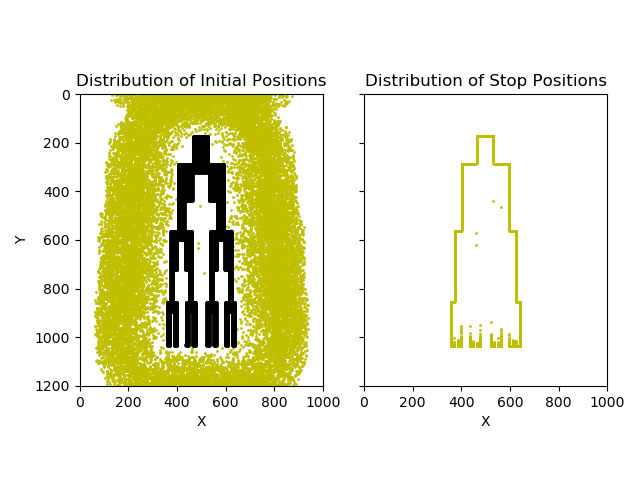
\includegraphics[width=\textwidth]{G_1_L_3_unwrap_disp_y_initial_pos_distribution.png}
         \caption{The irregular yellow domain consists of
           approximately one-fifth of particles whose starting sites
           in the simulation are more remote from the branching
           structure and closer to the borders of the
           image. Nevertheless, there still have a few particles
           between the branches. The yellow area has two notches near
           the top and bottom edge of the image resulting from the
           periodic boundary conditions. Similarly, yellow particles
           only can characterize the external boundary of the target
           object precisely.}
         \label{fig:G_1_L_3_disp_yellow_initial_pos_distribution}
        \end{figure}



        \begin{figure}
         \centering
         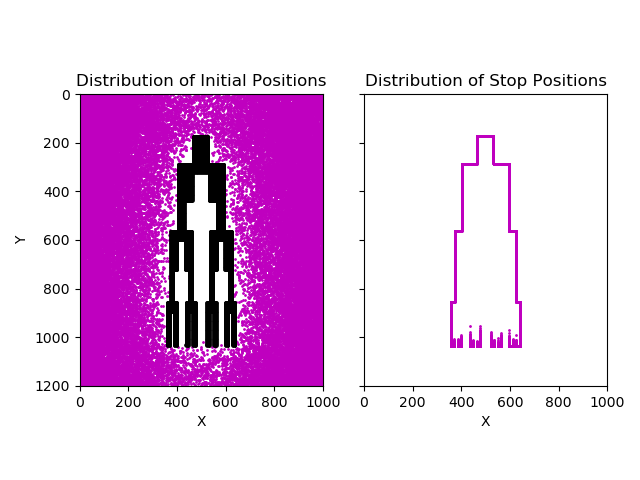
\includegraphics[width=\textwidth]{G_1_L_3_unwrap_disp_m_initial_pos_distribution.png}
         \caption{The rest of the particles fill the unoccupied space
           in the image, but none of them are localized between
           branches. Moreover, pink particles cannot explore the more
           detailed internal boundary of the branching structure
           compared with
           Fig.~\ref{fig:G_1_L_3_disp_yellow_initial_pos_distribution}.}
         \label{fig:G_1_L_3_disp_pink_initial_pos_distribution}
        \end{figure}


        

        \begin{figure}
        \centering
        \begin{subfigure}[b]{0.45\textwidth}
          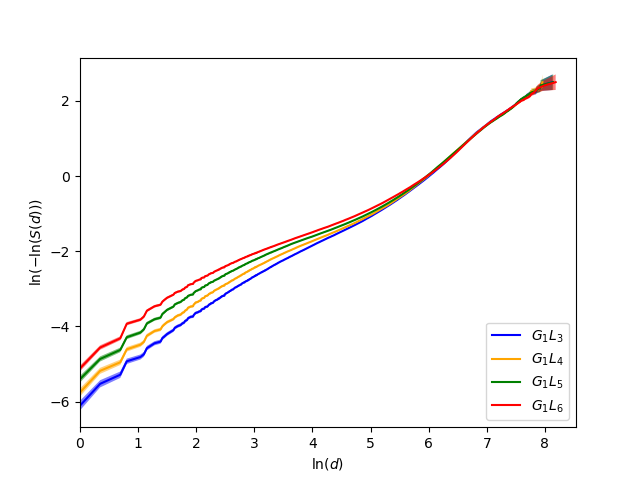
\includegraphics[width=\textwidth]{G_1_unwrap_disp_check_ph.png}
          \caption{}
          \label{fig:g1_disp_check_ph}
        \end{subfigure}
        \hfill
        \begin{subfigure}[b]{0.45\textwidth}
          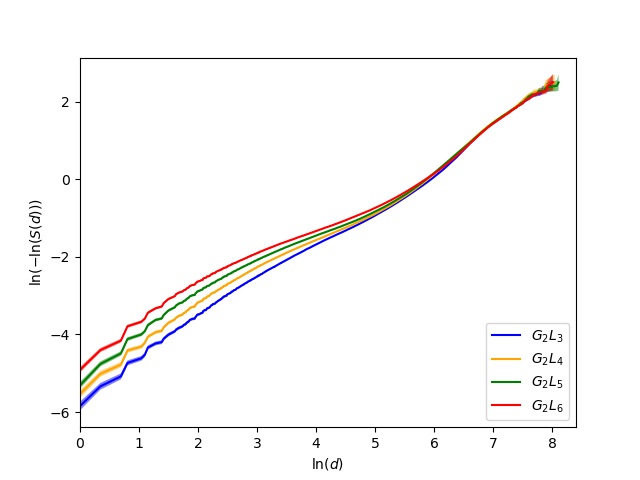
\includegraphics[width=\textwidth]{G_2_unwrap_disp_check_ph.png}
          \caption{}
          \label{fig:g1_disp_check_ph}
        \end{subfigure}
        \caption{}
        \label{fig:branch_disp_check_ph}
      \end{figure}

        
      

      \begin{table}
        \centering
        \begin{tabular}{llrrrr}
          \toprule
                       &             &         &  p &    &     \\
          \cmidrule{3-6}
                       &             & Logrank & TW & GB & FH  \\
          \midrule
          $G_1$ $L_3$  & $G_1$ $L_4$  &  0.0 &  0.0 &  0.0 &  0.0     \\
                       & $G_1$ $L_5$  & 0.0 & 0.0 & 0.0 & 0.0    \\
                       & $G_1$ $L_6$  & 0.0 & 0.0 & 0.0 & 0.0      \\
          $G_1$ $L_4$  & $G_1$ $L_5$  & 0.0072 & 0.0 & 0.0 & 0.0      \\
                       & $G_1$ $L_6$  & 0.0003 & 0.0 & 0.0 & 0.0       \\
          $G_1$ $L_5$   & $G_1$ $L_6$ & 0.2883 &  0.0 & 0.0 & 0.0      \\
          \bottomrule
        \end{tabular}
        \label{tab:g1_ingroup_tests_disp}
        \caption{}
      \end{table}


      \begin{table}
        \centering
        \begin{tabular}{llrrrr}
          \toprule
                       &             &         &  p &    &     \\
          \cmidrule{3-6}
                       &             & Logrank & TW & GB & FH  \\
          \midrule
          $G_2$ $L_3$  & $G_2$ $L_4$  &  0.0 &  0.0 &  0.0 &  0.0     \\
                       & $G_2$ $L_5$  & 0.0 & 0.0 & 0.0 & 0.0    \\
                       & $G_2$ $L_6$  & 0.0 & 0.0 & 0.0 & 0.0      \\
          $G_2$ $L_4$  & $G_2$ $L_5$  & 0.0001 & 0.0 & 0.0 & 0.0      \\
                       & $G_2$ $L_6$  & 0.0015 & 0.0 & 0.0 & 0.0       \\
          $G_2$ $L_5$   & $G_2$ $L_6$ & 0.7019 &  0.0 & 0.0 & 0.0      \\
          \bottomrule
        \end{tabular}
        \label{tab:g2_ingroup_tests_disp}
        \caption{}
      \end{table}



      

      \begin{figure}
        \centering
        \begin{subfigure}[b]{0.45\textwidth}
          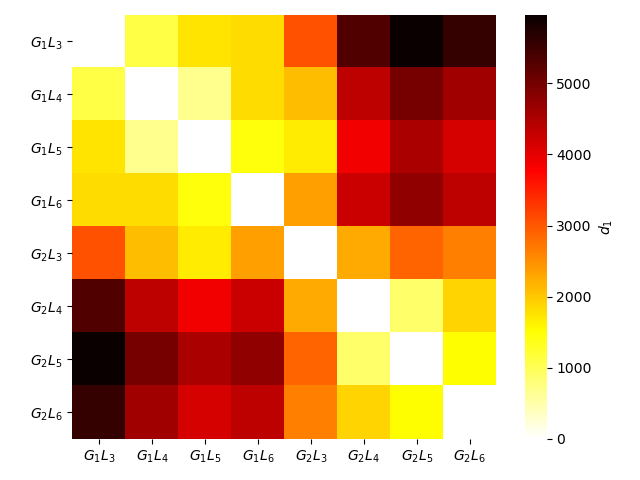
\includegraphics[width=\textwidth]{heatmap_ai_disp_l1.png}
          \caption{}
          \label{fig:heatmap_ai_disp_l1}
        \end{subfigure}
        \begin{subfigure}[b]{0.45\textwidth}
          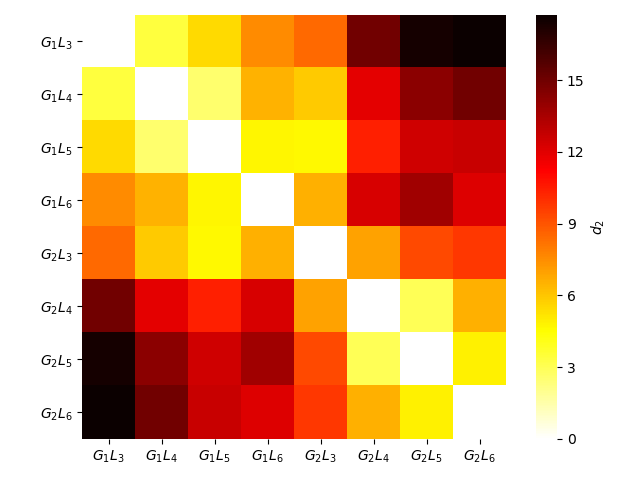
\includegraphics[width=\textwidth]{heatmap_ai_disp_l2.png}
          \caption{}
          \label{fig:heatmap_ai_disp_l2}
        \end{subfigure}
        \caption{}
        \label{fig:heatmap_ai_disp}
      \end{figure}
      
